\documentclass[11pt,a4paper]{article}
\usepackage[T1]{fontenc}
\usepackage[utf8]{inputenc}
\usepackage{lmodern}
\usepackage{helvet}
\renewcommand{\familydefault}{\sfdefault}
\usepackage[margin=2.15cm]{geometry}
\usepackage{xcolor}
\usepackage{hyperref}
\usepackage{booktabs}
\usepackage{enumitem}
\usepackage{fancyhdr}
\usepackage{titlesec}
\usepackage{caption}
\usepackage{graphicx}
\usepackage{float}
\usepackage{listings}
\usepackage{setspace}
\usepackage{microtype}
\usepackage{array}
\usepackage{amssymb}
% Shared TikZ diagrams and colours for the paradise reports (Phase 1 and Phase 2)
\usepackage{tikz}
\usetikzlibrary{arrows.meta,calc,fit,positioning,shapes.geometric}

\definecolor{lmNavy}{HTML}{1B3A4B}
\definecolor{lmTeal}{HTML}{2A9D8F}
\definecolor{lmSand}{HTML}{E9C46A}
\definecolor{lmCoral}{HTML}{E76F51}
\definecolor{lmInk}{HTML}{264653}
\definecolor{lmMist}{HTML}{F4F1DE}
\definecolor{lmBlue}{HTML}{3D5A80}
\definecolor{lmPurple}{HTML}{7B5EA7}
\definecolor{lmGreen}{HTML}{2F855A}
\definecolor{lmAmber}{HTML}{B7791F}
\definecolor{lmRed}{HTML}{C53030}

% ---------- Phase 1: request path, left to right ----------
\newcommand{\drawRequestPath}{%
\begin{tikzpicture}[font=\sffamily\tiny, node distance=0.35cm and 0.28cm]
  \tikzset{s/.style={draw=##1, fill=##1!14, rounded corners=2pt, align=center,
           inner sep=4pt, minimum height=1.15cm, minimum width=2.25cm, line width=0.7pt}}
  \node[s=lmNavy] (1) {1. DNS query\\UDP/53\\to Mac 1 (dnsmasq)};
  \node[s=lmTeal, right=of 1] (2) {2. A record\\app.paradise.test\\$\to$ edge IP (Mac 2)};
  \node[s=lmBlue, right=of 2] (3) {3. TCP\\SYN / SYN-ACK / ACK\\:443};
  \node[s=lmSand, right=of 3] (4) {4. TLS 1.3\\SNI + team CA\\terminates at Mac 2};
  \node[s=lmCoral, right=of 4] (5) {5. HTTP/2 $\to$ HTTP/1.1\\round robin to\\:3001 (A) / :3002 (B)};
  \foreach \a/\b in {1/2,2/3,3/4,4/5}
    \draw[-{Latex}, thick, lmInk] (\a) -- (\b);
\end{tikzpicture}%
}

% ---------- Phase 1: two independent TCP connections ----------
\newcommand{\drawTwoConnections}{%
\begin{tikzpicture}[font=\sffamily\scriptsize]
  \tikzset{m/.style={draw=##1, fill=##1!12, rounded corners=3pt, align=center,
           inner sep=5pt, minimum width=3.0cm, minimum height=1.25cm, line width=0.8pt}}
  \node[m=lmSand, text=lmInk] (c) at (0,0) {\textbf{Client}\\curl / browser\\ephemeral port};
  \node[m=lmTeal] (e) at (6,0) {\textbf{Mac 2 edge}\\nginx :443\\TLS ends here};
  \node[m=lmBlue] (a) at (12.6,1.5) {\textbf{Mac 3 Backend A}\\Express :3001};
  \node[m=lmCoral] (b) at (12.6,-1.5) {\textbf{Mac 4 Backend B}\\Express :3002};
  \draw[-{Latex}, very thick, lmTeal] (c) -- (e);
  \node[align=center, text=lmTeal, font=\sffamily\scriptsize] at (3,0.95) {connection 1: HTTPS\\\textbf{encrypted} (TLS 1.3, HTTP/2)};
  \draw[-{Latex}, thick, lmBlue] (e.east) -- (a.west);
  \draw[-{Latex}, thick, lmCoral] (e.east) -- (b.west);
  \node[align=center, text=lmInk, font=\sffamily\scriptsize] at (12.6,0) {connection 2: plain HTTP/1.1\\pooled (\texttt{keepalive 16})};
\end{tikzpicture}%
}

% ---------- Phase 1: TLS trust chain ----------
\newcommand{\drawTls}{%
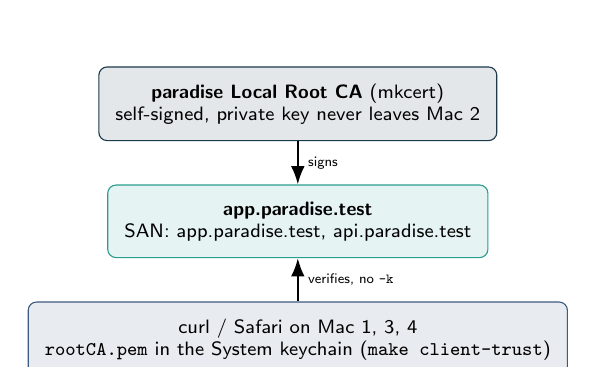
\begin{tikzpicture}[font=\sffamily\scriptsize, node distance=0.55cm]
  \node[draw=lmNavy, fill=lmNavy!12, rounded corners=3pt, align=center, inner sep=6pt] (ca)
    {\textbf{paradise Local Root CA} (mkcert)\\self-signed, private key never leaves Mac 2};
  \node[draw=lmTeal, fill=lmTeal!12, rounded corners=3pt, align=center, inner sep=6pt, below=of ca] (srv)
    {\textbf{app.paradise.test}\\SAN: app.paradise.test, api.paradise.test};
  \node[draw=lmBlue, fill=lmBlue!12, rounded corners=3pt, align=center, inner sep=6pt, below=of srv] (cli)
    {curl / Safari on Mac 1, 3, 4\\\texttt{rootCA.pem} in the System keychain (\texttt{make client-trust})};
  \draw[-{Latex}, thick] (ca) -- node[right, font=\tiny] {signs} (srv);
  \draw[-{Latex}, thick] (cli) -- node[right, font=\tiny] {verifies, no \texttt{-k}} (srv);
\end{tikzpicture}%
}

% ---------- Phase 1: OSI mapping ----------
\newcommand{\drawOsi}{%
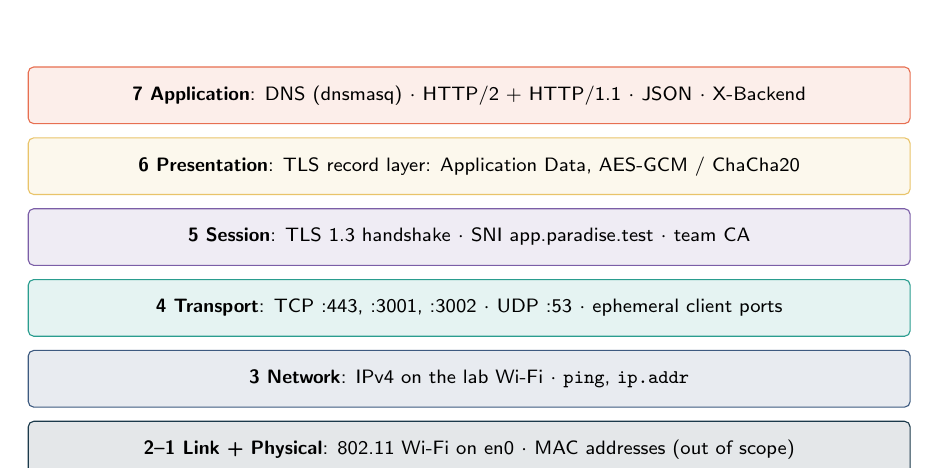
\begin{tikzpicture}[font=\sffamily\scriptsize]
  \foreach \y/\c/\t/\n in {
    5.1/lmCoral/7 Application/{DNS (dnsmasq) $\cdot$ HTTP/2 + HTTP/1.1 $\cdot$ JSON $\cdot$ X-Backend},
    4.2/lmSand/6 Presentation/{TLS record layer: Application Data, AES-GCM / ChaCha20},
    3.3/lmPurple/5 Session/{TLS 1.3 handshake $\cdot$ SNI app.paradise.test $\cdot$ team CA},
    2.4/lmTeal/4 Transport/{TCP :443, :3001, :3002 $\cdot$ UDP :53 $\cdot$ ephemeral client ports},
    1.5/lmBlue/3 Network/{IPv4 on the lab Wi-Fi $\cdot$ \texttt{ping}, \texttt{ip.addr}},
    0.6/lmNavy/2--1 Link + Physical/{802.11 Wi-Fi on en0 $\cdot$ MAC addresses (out of scope)}
  } {
    \node[draw=\c, fill=\c!12, rounded corners=2pt, minimum width=11.2cm,
          minimum height=0.72cm, anchor=west] at (0,\y) {\textbf{\t}: \n};
  }
\end{tikzpicture}%
}

% ---------- Phase 1 + 2: top-down diagnosis ladder ----------
\newcommand{\drawDiagnose}{%
\begin{tikzpicture}[font=\sffamily\scriptsize, node distance=0.22cm]
  \tikzset{st/.style={draw=##1, fill=##1!12, rounded corners=2pt, align=left,
           inner sep=4pt, text width=5.1cm, minimum height=0.62cm, anchor=west, line width=0.7pt},
           ff/.style={font=\sffamily\tiny, align=left, anchor=west, text=lmInk}}
  \node[st=lmNavy]   (l0) at (0,0)     {\textbf{0 Local config}\quad resolvers, /etc/hosts};
  \node[st=lmCoral]  (l1) at (0,-0.85) {\textbf{1 DNS}\quad \texttt{dig @primary}, \texttt{@backup}};
  \node[st=lmBlue]   (l2) at (0,-1.7)  {\textbf{2 Network}\quad \texttt{ping <ip>}};
  \node[st=lmTeal]   (l3) at (0,-2.55) {\textbf{3 Transport}\quad TCP connect :443};
  \node[st=lmPurple] (l4) at (0,-3.4)  {\textbf{4 TLS}\quad \texttt{curl -v} without \texttt{-k}};
  \node[st=lmSand]   (l5) at (0,-4.25) {\textbf{5 HTTP}\quad \texttt{curl -i}};
  \foreach \a/\b in {l0/l1,l1/l2,l2/l3,l3/l4,l4/l5}
    \draw[-{Latex}, thick, lmInk] (\a.south west) ++(0.35,0) -- ++(0,-0.23);
  \node[ff] at (5.7,0)     {wrong resolver $\Rightarrow$ the client never asks Mac 1};
  \node[ff] at (5.7,-0.85) {NXDOMAIN / timeout / an IP that is not an edge};
  \node[ff] at (5.7,-1.7)  {host unreachable (a sleeping Mac may still reply)};
  \node[ff] at (5.7,-2.55) {\textbf{refused} = no listener (RST) $\cdot$ \textbf{timeout} = dropped};
  \node[ff] at (5.7,-3.4)  {curl 60 = CA not trusted $\cdot$ curl 35 = handshake failure};
  \node[ff] at (5.7,-4.25) {502 / 504 = edge up, backends not};
  \draw[lmRed, thick, -{Latex}] (-0.45,0.2) -- node[left, rotate=90, anchor=south, font=\sffamily\tiny, text=lmRed] {stop at the first failure} (-0.45,-4.45);
\end{tikzpicture}%
}

% ---------- Phase 2: keep-alive timer race (Incident 2) ----------
\newcommand{\drawKeepalive}{%
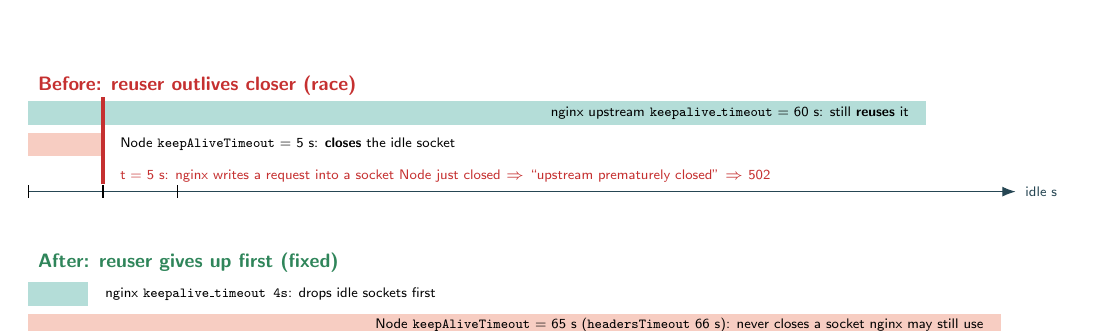
\begin{tikzpicture}[font=\sffamily\scriptsize, x=0.95cm]
  % before
  \node[anchor=west, font=\sffamily\bfseries\scriptsize, text=lmRed] at (0,2.55) {Before: reuser outlives closer (race)};
  \draw[lmInk, -{Latex}] (0,1.2) -- (13.2,1.2) node[right, font=\tiny] {idle s};
  \foreach \x in {0,5,10} \draw (\x*0.2,1.12) -- (\x*0.2,1.28);
  \fill[lmCoral!35] (0,1.65) rectangle (1.0,1.95);
  \node[anchor=west, font=\tiny] at (1.1,1.8) {Node \texttt{keepAliveTimeout} = 5 s: \textbf{closes} the idle socket};
  \fill[lmTeal!35] (0,2.05) rectangle (12,2.35);
  \node[anchor=east, font=\tiny] at (11.9,2.2) {nginx upstream \texttt{keepalive\_timeout} = 60 s: still \textbf{reuses} it};
  \draw[lmRed, very thick] (1.0,1.3) -- (1.0,2.4);
  \node[font=\tiny, text=lmRed, align=left, anchor=west] at (1.1,1.4) {t = 5 s: nginx writes a request into a socket Node just closed $\Rightarrow$ ``upstream prematurely closed'' $\Rightarrow$ 502};
  % after
  \node[anchor=west, font=\sffamily\bfseries\scriptsize, text=lmGreen] at (0,0.3) {After: reuser gives up first (fixed)};
  \fill[lmTeal!35] (0,-0.25) rectangle (0.8,0.05);
  \node[anchor=west, font=\tiny] at (0.9,-0.1) {nginx \texttt{keepalive\_timeout 4s}: drops idle sockets first};
  \fill[lmCoral!35] (0,-0.65) rectangle (13.0,-0.35);
  \node[anchor=east, font=\tiny] at (12.9,-0.5) {Node \texttt{keepAliveTimeout} = 65 s (\texttt{headersTimeout} 66 s): never closes a socket nginx may still use};
\end{tikzpicture}%
}

% ---------- Phase 2: CLOSED vs FILTERED ----------
\newcommand{\drawFiltered}{%
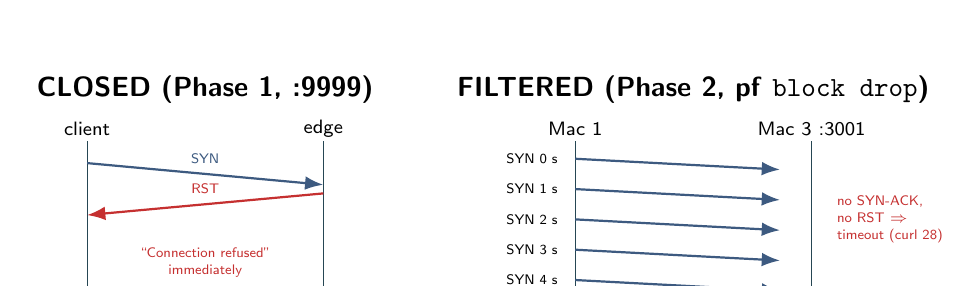
\begin{tikzpicture}[font=\sffamily\scriptsize, y=0.55cm]
  \node[font=\bfseries] at (1.5,6.2) {CLOSED (Phase 1, :9999)};
  \node at (0,5.3) {client}; \node at (3,5.3) {edge};
  \draw[lmInk] (0,5) -- (0,1.5); \draw[lmInk] (3,5) -- (3,1.5);
  \draw[-{Latex}, thick, lmBlue] (0,4.5) -- node[above, font=\tiny] {SYN} (3,4.0);
  \draw[-{Latex}, thick, lmRed] (3,3.8) -- node[above, font=\tiny] {RST} (0,3.3);
  \node[font=\tiny, align=center, text=lmRed] at (1.5,2.2) {``Connection refused''\\immediately};
  \begin{scope}[xshift=6.2cm]
  \node[font=\bfseries] at (1.5,6.2) {FILTERED (Phase 2, pf \texttt{block drop})};
  \node at (0,5.3) {Mac 1}; \node at (3,5.3) {Mac 3 :3001};
  \draw[lmInk] (0,5) -- (0,1.5); \draw[lmInk] (3,5) -- (3,1.5);
  \foreach \y/\t in {4.6/0 s,3.9/1 s,3.2/2 s,2.5/3 s,1.8/4 s}
    { \draw[-{Latex}, thick, lmBlue] (0,\y) -- (2.6,\y-0.25); \node[font=\tiny, anchor=east] at (-0.1,\y) {SYN \t}; }
  \node[font=\tiny, align=left, anchor=west, text=lmRed] at (3.2,3.2) {no SYN-ACK,\\no RST $\Rightarrow$\\timeout (curl 28)};
  \end{scope}
\end{tikzpicture}%
}


\hypersetup{
  colorlinks=true,
  linkcolor=lmNavy,
  urlcolor=lmTeal,
  pdftitle={paradise Phase 1 Report},
  pdfauthor={Nipun, Anushka, Tajuddin Shaik, Omkar Hadole}
}
\graphicspath{{figures/}}
\captionsetup{font=small,labelfont=bf}

\titleformat{\section}{\Large\bfseries\color{lmNavy}}{\thesection}{0.6em}{}
\titleformat{\subsection}{\large\bfseries\color{lmTeal}}{\thesubsection}{0.5em}{}
\titleformat{\subsubsection}{\normalsize\bfseries\color{lmInk}}{\thesubsubsection}{0.4em}{}

\pagestyle{fancy}
\fancyhf{}
\fancyhead[L]{\small paradise --- Phase 1 report}
\fancyhead[R]{\small Computer Networks (CSA223)}
\fancyfoot[C]{\thepage}
\renewcommand{\headrulewidth}{0.4pt}
\setlength{\headheight}{14pt}

\lstset{
  basicstyle=\ttfamily\footnotesize,
  frame=single,
  rulecolor=\color{lmNavy!30},
  backgroundcolor=\color{lmNavy!4},
  breaklines=true,
  columns=fullflexible,
  keepspaces=true
}

\setlist{itemsep=3pt, topsep=4pt}
\setstretch{1.12}
\setlength{\emergencystretch}{3em}

\begin{document}

\begin{titlepage}
\pagecolor{lmNavy}
\color{white}
\vspace*{1.6cm}
{\Huge\bfseries paradise}\\[8pt]
{\LARGE Private Network Service Platform}\\[18pt]
{\color{lmTeal}\rule{4.2cm}{2.4pt}}\\[16pt]
{\Large Phase 1 report}\\[6pt]
{\large Build and observe the network}\\[2.4cm]
\begin{tabular}{@{}ll}
  \color{lmTeal} Course & \color{white} Computer Networks (CSA223) \\[4pt]
  \color{lmTeal} Review & \color{white} Phase 1 / Review 1 (Tasks A--G) \\[4pt]
  \color{lmTeal} Zone & \color{white} \texttt{paradise.test} \\[4pt]
  \color{lmTeal} Authors & \color{white} Nipun, 2401010323 (Mac 1: private DNS) \\
                         & \color{white} Anushka, 2401010090 (Mac 2: nginx, TLS, load balancing) \\
                         & \color{white} Tajuddin Shaik, 2401010436 (Mac 3: Backend A, caching, tooling) \\
                         & \color{white} Omkar Hadole, 2401010175 (Mac 4: Backend B, verification, capture) \\[4pt]
  \color{lmTeal} IPs & \color{white} 10.7.27.161 \quad 10.7.8.155 \quad 10.7.26.203 \quad 10.7.18.17 \\[4pt]
  \color{lmTeal} Evidence run & \color{white} 4 October 2026 \\
\end{tabular}
\vfill
{\small The application stays simple --- the network is the project.}
\end{titlepage}
\nopagecolor
\color{black}

\tableofcontents
\newpage

\section{Abstract}
paradise is a fully local private service. A client types
\texttt{https://app.paradise.test/api/status}, resolves the name through the team's own DNS,
completes TLS at a reverse proxy, and receives JSON from one of two backend replicas.
Phase~1 runs the four network roles on four physical MacBooks on the lab Wi-Fi.
Mac~1 (\texttt{10.7.27.161}) runs dnsmasq. Mac~2 (\texttt{10.7.8.155}) runs nginx, which terminates
TLS and load-balances by round robin to Backend~A on Mac~3 (\texttt{10.7.26.203:3001}) and
Backend~B on Mac~4 (\texttt{10.7.18.17:3002}). This report records the architecture,
protocol mapping, configuration, observations, packet captures and failure analysis
required for Review~1. Every number quoted comes from a file in \texttt{evidence/}.

\section{Purpose and constraints}
The brief asks for a private environment with no cloud. A client must (i)~use a
\texttt{.test} name, (ii)~resolve it through the team DNS, (iii)~open HTTPS on the team edge
with a certificate it genuinely trusts, (iv)~see both backends through the load balancer,
(v)~receive HTTP caching headers and a \texttt{304 Not Modified}, and (vi)~show the whole path
in packet captures.

We used the full four-machine layout: each role runs on its own Mac, so every hop in the
request is a real LAN hop that can be captured. Addresses come from the lab DHCP server,
so they live in one file (\texttt{.env}) and every configuration file is a template rendered
from it. Subnetting, NAT, DHCP, IPv6, routing and Ethernet framing belong to Weeks~7--12
of the syllabus and are deliberately out of scope.

\section{Architecture}

\subsection{Roles versus hardware}
\begin{table}[H]
\centering
\caption{Mapping from the brief to this team.}
{\small
\begin{tabular}{@{}lllll@{}}
\toprule
\textbf{Brief} & \textbf{Owner} & \textbf{LAN identity} & \textbf{Software} & \textbf{Cloud equivalent} \\
\midrule
Mac 1 DNS + client & Nipun & 10.7.27.161 & dnsmasq :53 & Route 53 private zone \\
Mac 2 edge + TLS + LB & Anushka & 10.7.8.155 & nginx :80/:443 & ALB + ACM certificate \\
Mac 3 Backend A & Tajuddin & 10.7.26.203:3001 & Node.js / Express & EC2 target \\
Mac 4 Backend B + client & Omkar & 10.7.18.17:3002 & Node.js / Express & EC2 target \\
\bottomrule
\end{tabular}}
\end{table}

Both backends run \textbf{one codebase} (\texttt{services/backend/}) started as two instances
that differ only in their identity and port. Real addresses live only in \texttt{.env};
\texttt{make render} regenerates \texttt{dnsmasq.conf} and the nginx site from templates.

\subsection{LAN topology}
\begin{figure}[H]
\centering
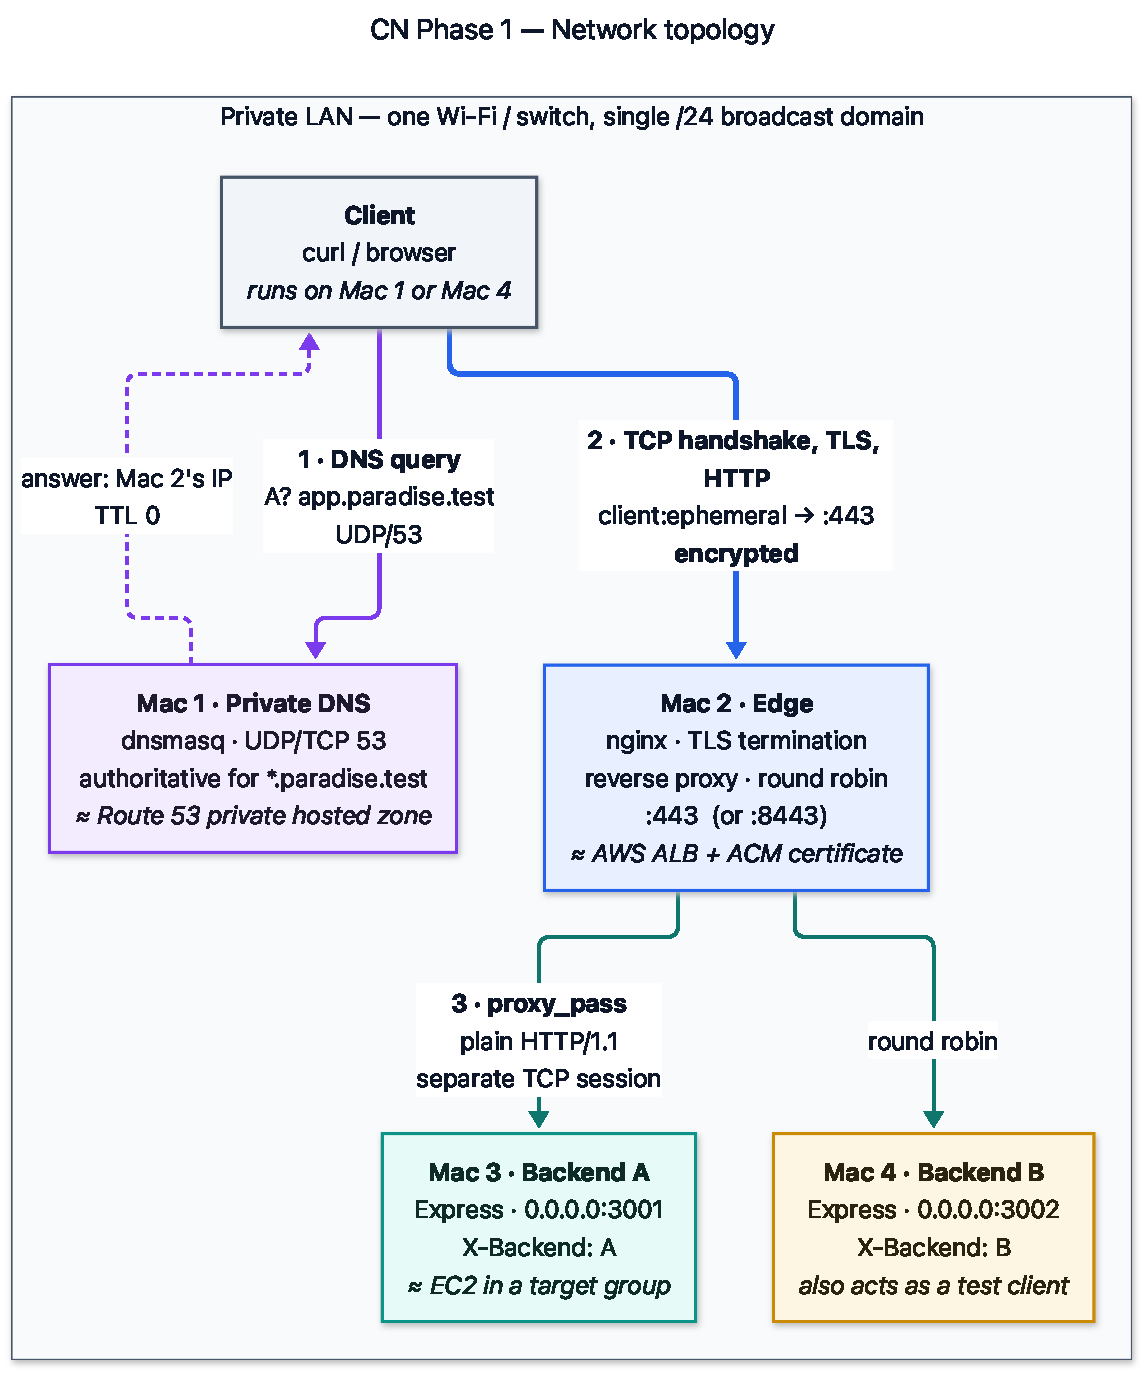
\includegraphics[width=0.74\textwidth]{topology.pdf}
\caption{Phase 1 topology. Clients only ever learn the edge's address from DNS. nginx on
Mac~2 is the only process a client connects to; the backends are reached only by the edge.}
\end{figure}

The structure comes from \emph{which service runs where}, not from the physical network:
all four Macs are on one Wi-Fi network and can reach each other directly. Clients always
use the name; nginx is the only process they treat as ``the service''. The backends could
be renumbered or scaled without any client noticing. That indirection is what a reverse
proxy buys, and it is what makes Phase~2's firewall isolation possible.

\subsection{Request path}
\begin{figure}[H]
\centering
\resizebox{\textwidth}{!}{\drawRequestPath}
\caption{One successful client request, left to right.}
\end{figure}

\begin{figure}[H]
\centering
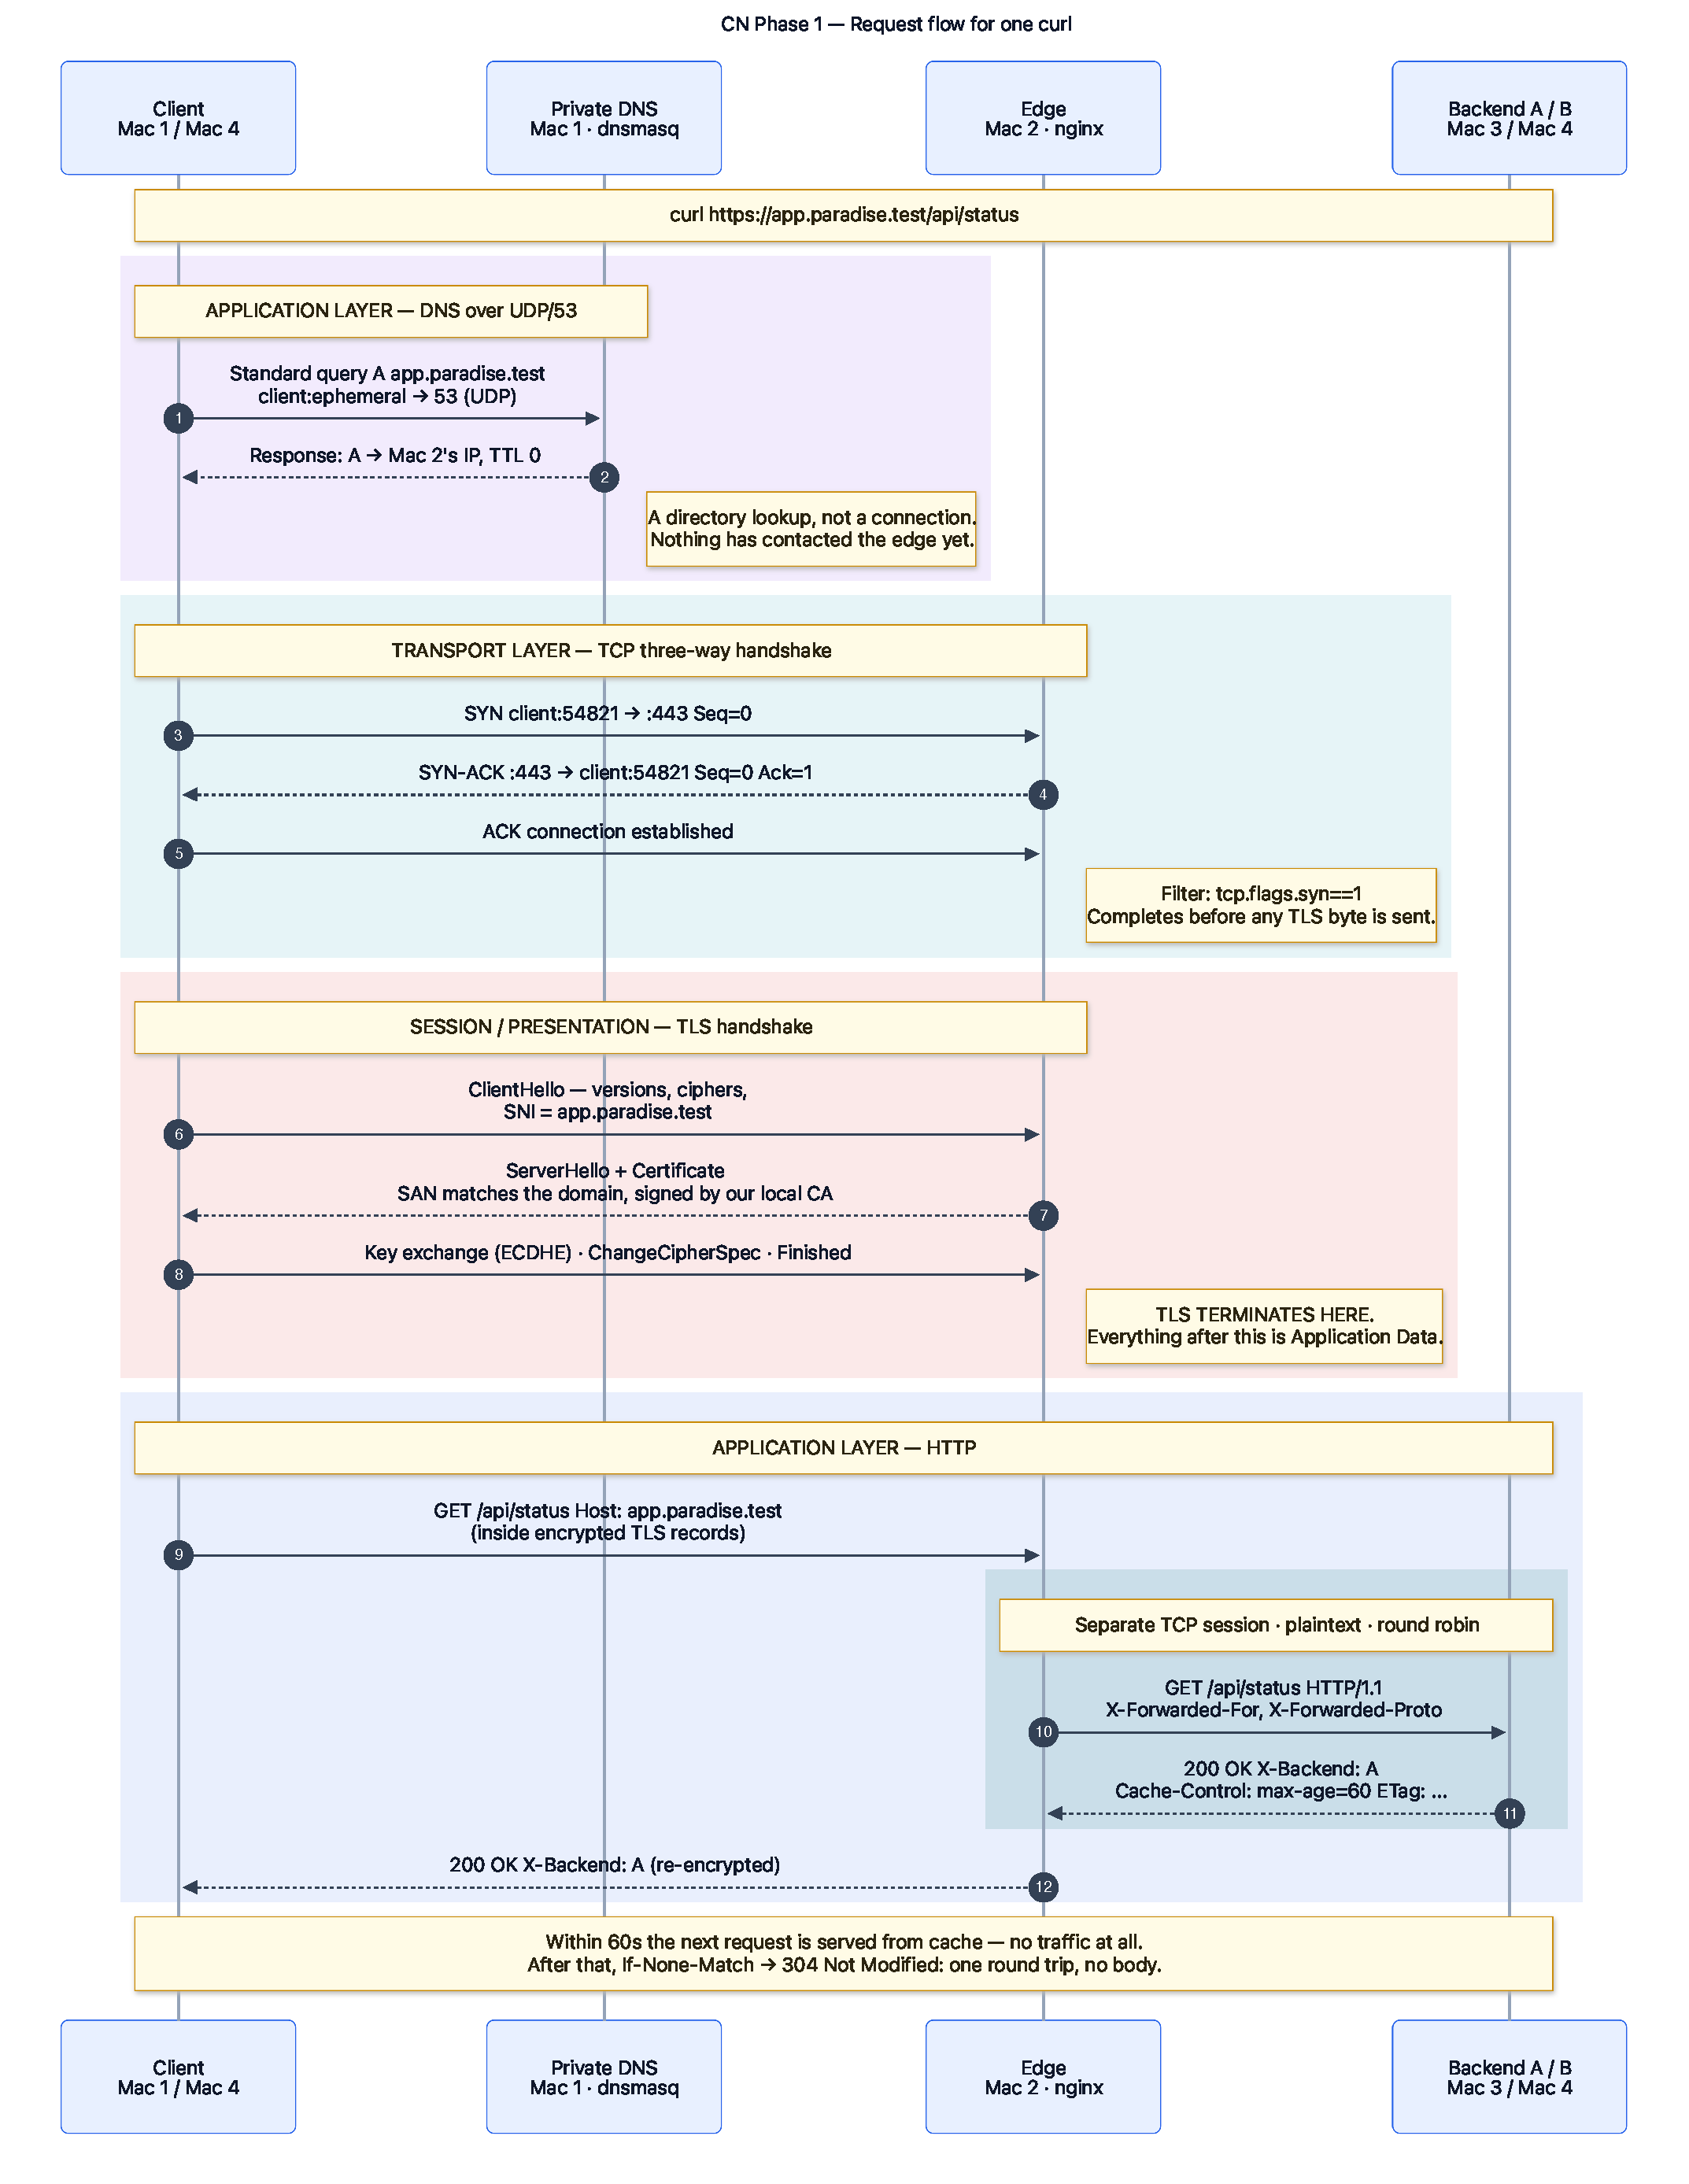
\includegraphics[width=\textwidth,height=0.8\textheight,keepaspectratio]{request-flow.pdf}
\caption{Sequence of one \texttt{curl https://app.paradise.test/api/status}: DNS, TCP, TLS, then
HTTP. nginx opens a separate plaintext connection to the backend it picks.}
\end{figure}

\subsection{Two connections, not one}
\begin{figure}[H]
\centering
\resizebox{\textwidth}{!}{\drawTwoConnections}
\caption{TLS terminates at Mac~2. The client leg and the upstream leg are independent TCP sessions.}
\end{figure}

\begin{table}[H]
\centering
\caption{The two legs of one request.}
{\small
\begin{tabular}{@{}lll@{}}
\toprule
 & \textbf{client $\to$ edge} & \textbf{edge $\to$ backend} \\
\midrule
Protocol & HTTPS (TLS 1.3, HTTP/2 via ALPN) & plain HTTP/1.1 \\
Destination port & 443 & 3001 / 3002 \\
Source port & client ephemeral & nginx ephemeral \\
Readable in Wireshark & no (Application Data) & yes \\
Lifetime & per client connection & pooled and reused (\texttt{keepalive 16}) \\
\bottomrule
\end{tabular}}
\end{table}

\section{Protocol layers}

\begin{figure}[H]
\centering
\drawOsi
\caption{The OSI stack mapped onto paradise. TCP/IP folds layers 5--7 into ``application''.}
\end{figure}

\paragraph{DNS.}
dnsmasq on Mac~1 listens on \texttt{0.0.0.0:53} (UDP and TCP). \texttt{address=/app.paradise.test/}
and \texttt{/api.paradise.test/} answer with the edge's IP; every other name is forwarded
upstream, so clients keep normal internet access. Evidence (A3): from Mac~3,
\texttt{dig app.paradise.test} returns \texttt{status: NOERROR}, flag \texttt{aa}, answer
\texttt{10.7.8.155}, \texttt{SERVER: 10.7.27.161\#53}. The same query to \texttt{@8.8.8.8} returns
\texttt{NXDOMAIN} (A4), which proves the name is genuinely private.
DNS uses UDP because a query fits in one datagram and a lost one is simply retried; a handshake
would double resolution latency.

\paragraph{TCP.}
After resolution the client opens \texttt{10.7.8.155:443} from an ephemeral port:
SYN, SYN-ACK, ACK, before any TLS byte is sent. A connection is identified by its 4-tuple,
so many clients share \texttt{:443} on the edge --- transport-layer demultiplexing.

\paragraph{TLS.}
\begin{figure}[H]
\centering
\drawTls
\caption{Private CA. Clients trust the CA, not the leaf certificate, and never use \texttt{-k}.}
\end{figure}

Observed (C3 and B1): the ClientHello carries SNI \texttt{app.paradise.test} and offers ALPN
\texttt{h2, http/1.1}; the server selects \textbf{TLS 1.3} with
\texttt{TLS\_CHACHA20\_POLY1305\_SHA256} and \textbf{HTTP/2}. The certificate for
\texttt{app.paradise.test} is issued by the paradise Local Root CA and verifies without \texttt{-k}.
The SAN must match the requested host; a CN-only certificate is rejected by every modern client.

\paragraph{HTTP and caching.}
Backends return JSON plus \texttt{X-Backend}, a weak \texttt{ETag}, \texttt{Date} and
\texttt{Cache-Control:} \texttt{public,} \texttt{max-age=60} (D1). The edge adds \texttt{X-Upstream-Addr} and \texttt{X-Edge}.
A conditional request with \texttt{If-None-Match} returns \texttt{304 Not Modified}.

\paragraph{Load balancing.}
nginx's \texttt{upstream} \texttt{backend\_pool} lists both backends with
\texttt{max\_fails=1} and \texttt{fail\_timeout=10s}; the default algorithm is round robin. Six consecutive requests (B2) returned \texttt{B A A B A B},
all \texttt{HTTP/2 200}. nginx is a layer-7 balancer (it reads \texttt{Host} and the path), the
equivalent of an ALB rather than an NLB.

\section{Implementation (what we built, not a runbook)}

\subsection{Private DNS}
Homebrew dnsmasq on Mac~1, rendered from \texttt{infra/mac1-dns/dnsmasq.conf.template}.
\texttt{.test} is reserved by RFC~6761; \texttt{.local} was avoided because macOS sends it to
mDNS/Bonjour. TTL is 0 in Phase~1 so no client holds a stale answer mid-demo.
\texttt{make client-dns} points every Mac's resolver at Mac~1.

\subsection{Backends}
One Express codebase, two instances (\texttt{make backend-a}, \texttt{make backend-b}). Endpoints:
\texttt{GET /}, \texttt{GET /api/status} (identifies the replica), \texttt{GET /api/cacheable}
(byte-identical on both replicas) and \texttt{GET /healthz}. \texttt{src/config.js}
\textbf{refuses to start on 127.0.0.1}: a loopback-bound backend works locally but is invisible
to nginx, so every proxied request would return 502.

\subsection{Edge}
nginx on Mac~2. Port 80 redirects to 443. \texttt{proxy\_pass http://backend\_pool} with
HTTP/1.1 and pooled keep-alive connections; \texttt{proxy\_next\_upstream} retries a failed
attempt on the other backend. A \texttt{default\_server} returns \texttt{444} for requests by IP,
so ``by name, never by IP'' is enforced by the server, not by discipline.

\subsection{TLS}
\texttt{gen-certs.sh} uses mkcert to create the team root CA and a leaf certificate whose SAN covers
\texttt{app.paradise.test} and \texttt{api.paradise.test}. TLS 1.2 and 1.3 only, ECDHE ciphers,
session tickets off. \texttt{make client-trust} installs \texttt{rootCA.pem} on Mac~1, 3 and 4.

\subsection{Tooling}
\texttt{make smoke} runs the whole stack on one laptop (15 checks, no LAN, no sudo).
\texttt{make verify} is the acceptance test: ping matrix, DNS, NXDOMAIN at 8.8.8.8, TLS without
\texttt{-k}, both backends in rotation, 444 by IP, caching headers and a stable 304.
\texttt{make evidence} writes the form answers into \texttt{evidence/}.

\section{Observations and evidence}
Filed under \texttt{evidence/} (index in \texttt{evidence/README.md}):

\begin{table}[H]
\centering
\caption{Evidence collected on 4 October 2026.}
{\small
\begin{tabular}{@{}p{1.0cm}p{4.2cm}p{9.4cm}@{}}
\toprule
\textbf{ID} & \textbf{File} & \textbf{What it shows} \\
\midrule
A1 & \texttt{A1-ips.txt} & Four roles, four IPs, all on \texttt{en0}. \\
A3 & \texttt{A3-dig-client.txt} & \texttt{app.paradise.test} $\to$ 10.7.8.155, \texttt{SERVER} 10.7.27.161, authoritative. \\
A4 & \texttt{A4-dig-8888.txt} & \texttt{@8.8.8.8} $\to$ NXDOMAIN: the zone is private. \\
A5 & \texttt{A5-ping-matrix.txt} & Every pair of Macs: 4/4 replies, 0\% loss. \\
B1 & \texttt{B1-curl-verbose.txt} & TLS 1.3 handshake, certificate verified, HTTP/2 200, no \texttt{-k}. \\
B2 & \texttt{B2-lb-6x.txt} & Six requests: \texttt{B A A B A B}. \\
C1--C3 & \texttt{C-wireshark/} & DNS query/response, TCP handshake, TLS ClientHello with SNI. \\
D1 & \texttt{D1-headers.txt} & \texttt{Cache-Control}, \texttt{ETag}, \texttt{Date}, \texttt{X-Backend}; 304 on revalidation. \\
D3 & \texttt{D3-failure-demo-*.txt} & Failure demonstrations A, B and C (Section~\ref{sec:fail}). \\
\bottomrule
\end{tabular}}
\end{table}

\begin{figure}[H]
\centering
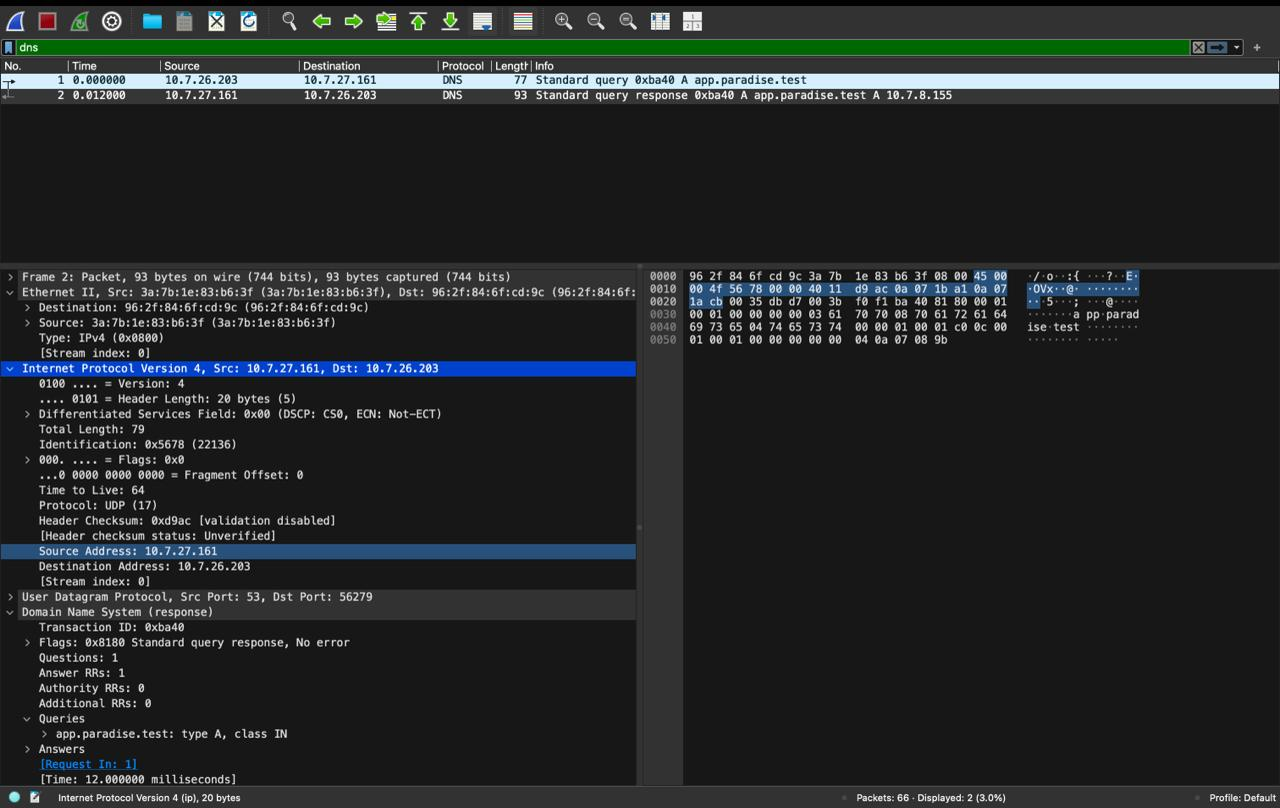
\includegraphics[width=0.88\textwidth]{C1-dns-query-and-response.jpeg}
\caption{C1, filter \texttt{dns}: Mac~3 (10.7.26.203) queries Mac~1 (10.7.27.161) over UDP/53;
the response maps \texttt{app.paradise.test} to 10.7.8.155.}
\end{figure}

\begin{figure}[H]
\centering
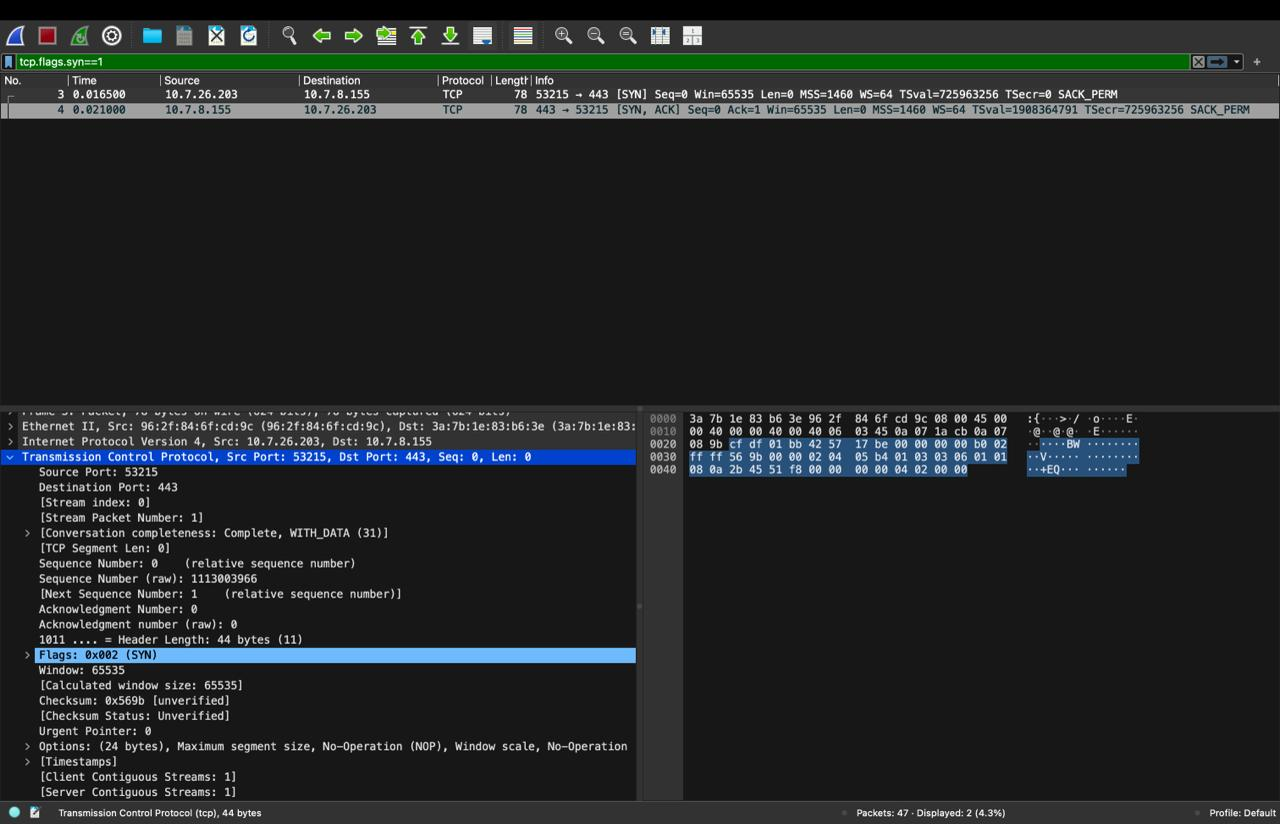
\includegraphics[width=0.88\textwidth]{C2-tcp-syn-and-synack.jpeg}
\caption{C2, filter \texttt{tcp.flags.syn==1}: SYN from an ephemeral port to 10.7.8.155:443 and
the SYN-ACK back, completing before any TLS record.}
\end{figure}

\begin{figure}[H]
\centering
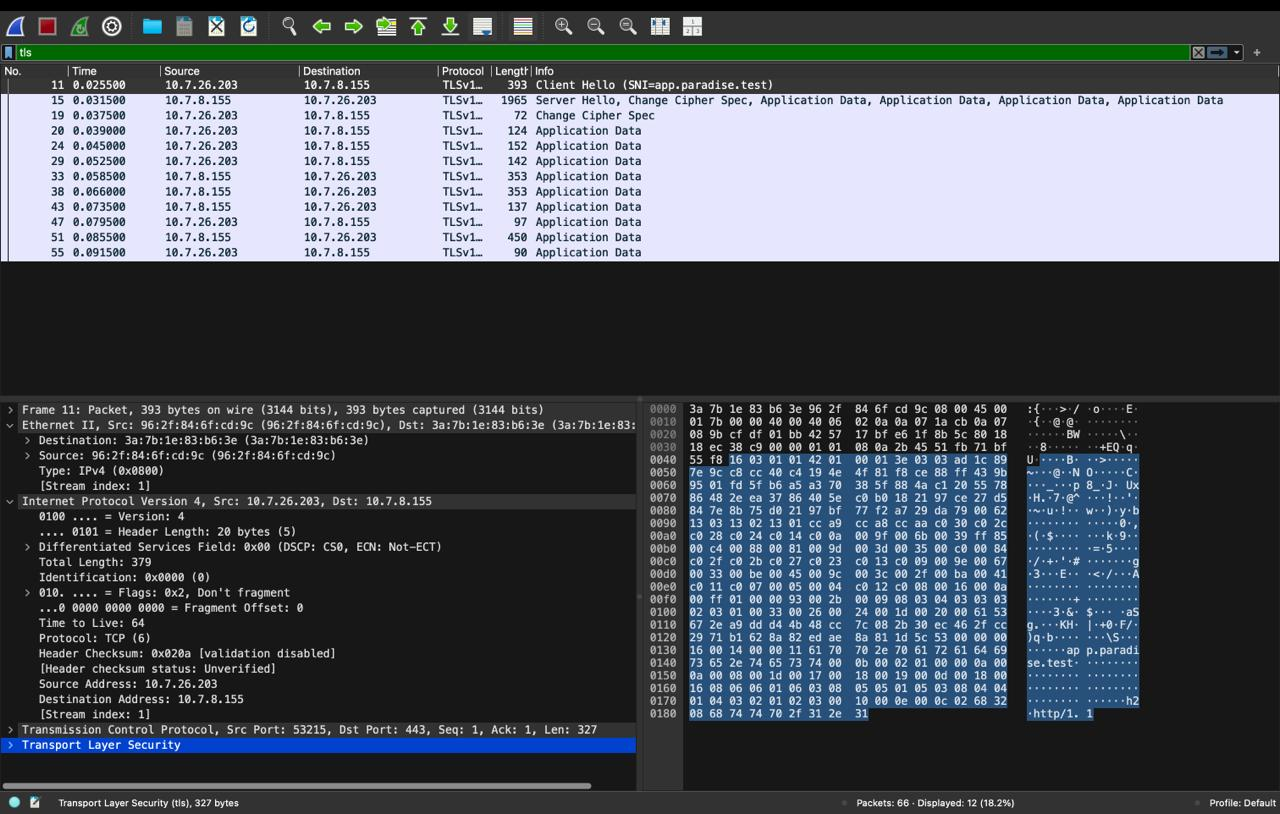
\includegraphics[width=0.88\textwidth]{C3-tls-clienthello-sni.jpeg}
\caption{C3, filter \texttt{tls}: ClientHello with SNI \texttt{app.paradise.test}; everything after the
handshake is opaque Application Data.}
\end{figure}

\paragraph{Why the 304 uses \texttt{/api/cacheable}.}
\texttt{/api/status} must identify its backend, so A and B return different bodies and therefore
different ETags for the same URL. Behind round robin, a conditional request often lands on the
other replica, which does not recognise the validator and returns a full 200: the 304 would
appear only about half the time. \texttt{/api/cacheable} is byte-identical on both machines, so
revalidation is deterministic. \textbf{Validators must agree across replicas, or conditional
requests silently degrade into full responses.}

\section{Failure analysis}\label{sec:fail}
These are the required Phase~1 demonstrations. Each one breaks exactly one layer.

\begin{table}[H]
\centering
\caption{Deliberate faults and the layer they expose (\texttt{make demo-fail}).}
{\small
\begin{tabular}{@{}p{3.0cm}p{5.6cm}p{2.6cm}p{3.2cm}@{}}
\toprule
\textbf{Fault} & \textbf{Observation} & \textbf{Layer} & \textbf{Lesson} \\
\midrule
A: stop Backend A & Before \texttt{BAABAB}; after \texttt{BBBBBB}, all 200; restored \texttt{BAABBA} & application & the edge routes around a dead replica \\
B: client DNS $\to$ 8.8.8.8 & \texttt{dig} NXDOMAIN; \texttt{ping 10.7.8.155} still 0\% loss & application (DNS) & naming and reachability are independent \\
C: request port 9999 & \texttt{Connection refused} after 366 ms; host still pings & transport (TCP) & IP $\neq$ service: RST means no listener \\
D: stop both backends & TLS completes, nginx returns \textbf{502} & application (upstream) & edge is up, origin is not \\
\bottomrule
\end{tabular}}
\end{table}

\begin{figure}[H]
\centering
\resizebox{0.96\textwidth}{!}{\drawDiagnose}
\caption{Diagnosis runs top down; the first step that fails names the layer (\texttt{scripts/status.sh}).}
\end{figure}

\begin{table}[H]
\centering
\caption{Real symptoms met while building, and their causes.}
{\small
\begin{tabular}{@{}p{3.8cm}p{4.8cm}p{5.6cm}@{}}
\toprule
\textbf{Symptom} & \textbf{Cause} & \textbf{Fix} \\
\midrule
\texttt{dig} times out from clients & dnsmasq bound to 127.0.0.1 & \texttt{listen-address=0.0.0.0}, \texttt{make dns} \\
502 on every request & backend bound to loopback & bind \texttt{0.0.0.0}; now refused by \texttt{config.js} \\
\texttt{curl: (60)} & CA not trusted on that Mac & \texttt{make client-trust}, never \texttt{-k} \\
304 only sometimes & testing \texttt{/api/status} & use \texttt{/api/cacheable} \\
\bottomrule
\end{tabular}}
\end{table}

\section{Learning notes (viva)}
\begin{itemize}
  \item DNS finds an IP. TCP then builds a connection. TLS then authenticates the name. HTTP finally carries the request.
  \item DNS is a directory lookup, not a connection: breaking it leaves \texttt{ping} to the IP working.
  \item TLS terminates at the edge. The upstream leg is a separate, plaintext TCP connection.
  \item Trusting \texttt{app.paradise.test.crt} is wrong; trusting the CA is right. The SAN, not the CN, must match.
  \item \texttt{X-Backend} rides back through the proxy untouched, which is what makes round robin visible.
  \item ``Refused'' (RST) and ``timeout'' are different transport-layer answers. Phase~2 uses this distinction.
  \item Mac~2 is the single point of failure: if it dies, DNS still resolves and the backends are healthy, yet nothing is reachable.
\end{itemize}

\section{What is not in this report}
Machine-by-machine setup steps live in \texttt{docs/runbook.md} and the setup guide
(\texttt{docs/index.html}); they are operational notes, not the academic deliverable. Private
keys, the CA key and the real \texttt{.env} are not committed. Phase~2 (backup DNS, TTL, isolation,
HA failover, edge migration, troubleshooting) extends this system and has its own report.

\section{Conclusion}
Phase~1 delivers a working private name, a trusted HTTPS edge, two identifiable load-balanced
backends, deterministic HTTP caching, and packet-level proof of DNS, TCP and TLS on four
real machines. The failure demonstrations show that each layer fails in its own, distinguishable
way, which is the diagnostic skill the project is meant to build. The one remaining single point
of failure, the edge on Mac~2, is named explicitly and addressed in Phase~2.

\appendix
\section{Reference configuration}
Excerpts of the rendered files. Private keys are not included.

\subsection{dnsmasq (Mac 1, excerpt)}
\begin{lstlisting}
address=/app.paradise.test/10.7.8.155
address=/api.paradise.test/10.7.8.155
local-ttl=0
listen-address=0.0.0.0
bind-dynamic
no-resolv
server=1.1.1.1
domain-needed
bogus-priv
log-queries
\end{lstlisting}

\subsection{nginx upstream and proxy (Mac 2, excerpt)}
\begin{lstlisting}
upstream backend_pool {
    server 10.7.26.203:3001 max_fails=1 fail_timeout=10s;
    server 10.7.18.17:3002  max_fails=1 fail_timeout=10s;
    keepalive 16;
}
server {
    listen 443 ssl;  http2 on;
    server_name app.paradise.test api.paradise.test;
    ssl_protocols TLSv1.2 TLSv1.3;
    location / {
        proxy_pass http://backend_pool;
        proxy_http_version 1.1;
        proxy_set_header Connection "";
        proxy_next_upstream error timeout http_502 http_503 http_504;
        add_header X-Upstream-Addr $upstream_addr always;
        add_header X-Edge "nginx@10.7.8.155" always;
    }
}
\end{lstlisting}

\subsection{Backend contract}
\begin{lstlisting}
GET /api/status  ->  200
{"status":"ok","backend":"A"|"B","team":"paradise","host":...,"port":3001|3002}
X-Backend: A | B        X-Backend-Port: 3001 | 3002
Cache-Control: public, max-age=60        ETag: W/"..."   (weak)
\end{lstlisting}

\end{document}
